\documentclass[18pt, aspectratio=169]{beamer}
% \documentclass{etp-beamer-fancy}
\usepackage[utf8]{inputenc}
\usepackage{templates/beamerthemekit}
\usepackage{graphicx}
\usepackage{microtype}
\usepackage{hyperref}
\usepackage{siunitx}
\usepackage{upgreek}
\usepackage{hepnames}
\usepackage{hepparticles}
\usepackage{appendixnumberbeamer}
\usepackage{booktabs}
\usepackage{subcaption}
\usepackage{blkarray}
\usepackage{tikz-feynman}
\usepackage{physics}

\title{Observation of $CP$ violation in charm decays}
\subtitle{Tracking Meeting}
\author[Michael Eliachevitch
(\href{mailto:michael.eliachevitch@kit.edu}{michael.eliachevitch@kit.edu})]{Michael Eliachevitch(\href{mailto:michael.eliachevitch@kit.edu}{michael.eliachevitch@kit.edu})}
\titleimage{quarksBig}
\titlelogo{belle2-logo}
\institute[ETP -- KIT]{Institut für Experimentelle Teilchenphysik (ETP) -- KIT}
\date{25 June 2019}

\newcommand{\kitemph}[1]{\textcolor{kit-green100}{\bf{#1}}}

\newcommand{\PDstarplus}{\HepParticle{D}{}{*+}}
\newcommand{\hh}{h^+h^-}

\begin{document}
\maketitle

\begin{frame}
  \frametitle{$CP$ violation in the Standard Model}
  \begin{columns}
    \begin{column}{.5\textwidth}
      \begin{itemize}
      \item $CP$-violation (CPV): breaking of the invariance with respect to the combined transformation \kitemph{charge
        conjugation ($C$)} and \kitemph{parity inversion ($P$)}
      \item Sakharov: theoretical requirement for \kitemph{baryon-asymmetry} of the universe
      \item arises in SM from a \textcolor{kit-red100}{non-vanishing complex phase} for a
        \kitemph{quark mixing} matrix with 3 (\kitemph{$V_{\rm CKM}$}) or more generations
      \item \kitemph{suppressed for charm}$\mathcal{O}(A_{CP}) = 10^{-4} - 10^{-3}$
      \end{itemize}
    \end{column}

    \begin{column}{.7\textwidth}
      \centering
      \includegraphics[width=0.5\textwidth]{figures/cp_application_feyn.pdf}
        \begin{equation*}
          \begin{blockarray}{cccc}
            \textcolor{kit-green100}{\Pdown} & \textcolor{kit-green100}{\Pstrange} & \textcolor{kit-green100}{\Pbottom}{} \\
            \begin{block}{(ccc)c}
              1                    & \lambda    & \lambda^3 e^{i\textcolor{kit-red100}{\phi}} & \textcolor{kit-green100}{\Pup}    \\
              -\lambda             & 1          & \lambda^2           & \textcolor{kit-green100}{\Pcharm} \\
              -\lambda^3 e^{-i\textcolor{kit-red100}{\phi}} & -\lambda^2 & 1                  & \textcolor{kit-green100}{\Ptop}   \\
            \end{block}
          \end{blockarray}
        \end{equation*}
        ($\lambda \approx 0.22$)
    \end{column}
  \end{columns}
\end{frame}

\begin{frame}
  \frametitle{Reminder: Different types of CPV}
  \begin{description}
  \item[\textbf{CPV in decay (direct):}]
   % \[\frac{\Gamma(M \rightarrow f)}{\Gamma(\bar{M} \rightarrow \bar{f})} =
   %   \frac{\abs{A_f}^2}{\abs{\bar{A}_\bar{f}}^2} \neq 1\]
    \[\Gamma(M \rightarrow f) \neq \Gamma(\bar{M} \rightarrow \bar{f})\]
 \item[\textbf{CPV from mixing (indirect)}]
   \[\Gamma(M^0 \rightarrow \bar{M}^0) \neq \Gamma(\bar{M}^0 \rightarrow M^0)\]
 \item[\textbf{CPV from interference of mixing and decay}]
   \[\Gamma(M^0 \rightarrow f_{CP}) \neq \Gamma(\bar{M}^0 \rightarrow f_{CP})\]
  \end{description}
\end{frame}

\begin{frame}
  \frametitle{Motivation: Why bother?}
  \begin{block}{CPV discoveries so far}
    \begin{description}
    \item[1956] Wu: Discovery of parity violation
    \item[1964] Cronin, Fitch: CPV in \PK decays (mixing)
    \item[1973] Kobayashi, Mask's: CKM matrix
    \item[1999] NA31/48, KTeV: Direct CPV in \PK decays
    \item[2001] BaBar and Belle: CPV in $\PBzero \rightarrow \PJpsi\PKshort$\\
      $\Rightarrow$ CPV well-established
    \end{description}
  \end{block}
  \pause
  \begin{exampleblock}{Motivation for charm studies}
    \begin{itemize}
    \item CPV \kitemph{too low in SM} to explain baryon-asymmetry\\
      $\rightarrow$ NP contributions?
    \item small SM CPV in charm $\rightarrow$ \kitemph{sensitive to NP}
    \item CPV with \kitemph{up-type quarks}
    \item theory challenge: low-energy QCD
    \end{itemize}
  \end{exampleblock}
\end{frame}

\begin{frame}
  \frametitle{The LHCb Experiment}
  \begin{columns}
    \begin{column}{0.45\textwidth}
      \begin{itemize}
      \item ``single-arm forward spectrometer''
      \item $pp$ @ \SI{13}{\TeV}: large cross-section for \PB and \PD-meson production
      \item large boosts $\rightarrow$ displaced vertices
      \item good PID capabilities
      \item analysis used \SI{5.9}{\per\femto\barn}
      \item triggers: 1 hardware, 2 software (``turbo stream'' online reco)
      \end{itemize}
    \end{column}
    \begin{column}{0.55\textwidth}
      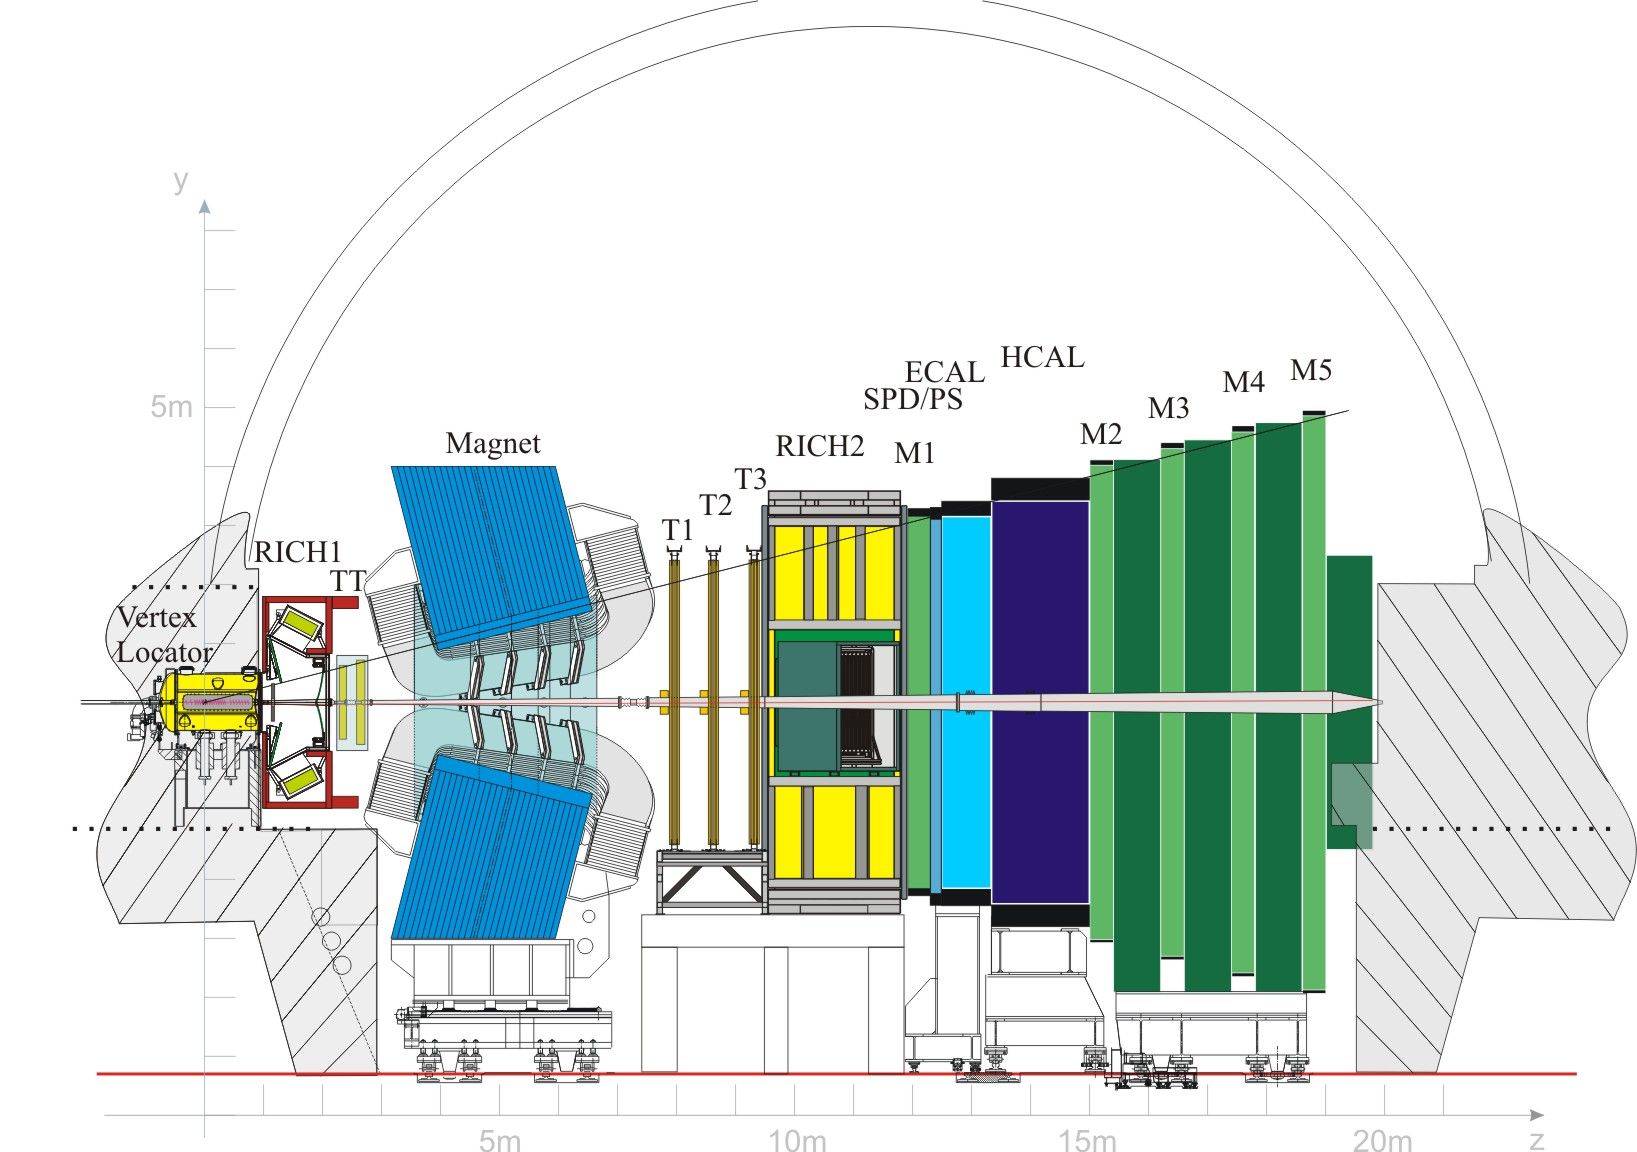
\includegraphics[width=\textwidth]{figures/Lhcbview.jpg}
    \end{column}
  \end{columns}

\end{frame}

\begin{frame}
  \frametitle{Tagged  $\PDzero \rightarrow \PKplus\PKminus/\Ppiplus\Ppiminus$ decays at LHCb}
  \begin{columns}
    \begin{column}{.5\textwidth}
      \centering
      \includegraphics[width=.5\textwidth]{figures/D0_to_hh_decays_at_lhcb_pitagged.pdf}\\
      \textbf{\Ppi tagged}\\
      \begin{itemize}
      \item prompt decays $\PDstarplus \rightarrow \Ppiplus\PDzero(\rightarrow h^+h^-)$
      \item kaons/pions from \PDzero form displaced vertex
      \item pion charge determines flavor, forms \PDstarplus vertex at primary vertex
      \end{itemize}
    \end{column}

    \begin{column}{.5\textwidth}
      \centering
      \includegraphics[width=.6\textwidth]{figures/D0_to_hh_decays_at_lhcb_mutagged.pdf}\\
      \textbf{\Pgm tagged}\\
      \begin{itemize}
      \item semileptonic \PB decays $\PBminus \rightarrow \Pgm\APnum\PDzero(\rightarrow h^+h^-)$
      \item muon paired with \PDzero at displaced vertex tags flavor
      \item $m_{\rm corr}$ is the \PDzero\Pmuon mass corrected for the missing neutrino $p_T$
      \end{itemize}
    \end{column}
  \end{columns}
\end{frame}

\begin{frame} \frametitle{Measuring charge asymmetry}
\begin{itemize}
\item CP asymmetry (time-integrated)
\begin{equation*}
  \textcolor{kit-green100}{A_{CP}(\PDzero \rightarrow \hh)} = \frac{\Gamma(\PDzero \rightarrow \hh) - \Gamma(\APDzero \rightarrow \hh)}{\Gamma(\PDzero \rightarrow \hh) + \Gamma(\APDzero \rightarrow \hh)}
\end{equation*}
\item Raw measured asymmetry
  \begin{eqnarray*}
  A_{\rm raw}(\PDzero \rightarrow \hh) & = & \frac{N(\PDzero \rightarrow \hh) - N(\APDzero \rightarrow
                                         \hh)}{N(\PDzero \rightarrow \hh) + N(\APDzero \rightarrow
                                         \hh)}\\
                                       & \approx & \textcolor{kit-green100}{A_{CP}(\PDzero \rightarrow \hh)} + \textcolor{kit-red100}{A_D(\Ppi/\Pmu)}
                                                   + \textcolor{kit-blue100}{A_P(\PDstar/\PBminus)}
  \end{eqnarray*}
  \begin{itemize}
  \item \textcolor{kit-red100}{$A_D$ detection asymmetries:} charge-dependent reconstruction
    efficiencies for pions/muons
  \item \textcolor{kit-blue100}{$A_P$ production asymmetries:} from hadronization asymmetries of \PDstar and
    \Pbottom in $pp$-collisions
  \end{itemize}
\end{itemize}
\end{frame}

\begin{frame}
  \frametitle{What is measured: $\Delta A_{CP}$}
  \begin{itemize}
  \item detection and production asymmetries \kitemph{cancel in difference}
    \textcolor{kit-green100}{
    \begin{eqnarray*}
      \Delta A_{CP} & = & A_{CP}(\PKplus\PKminus) - A_{CP}(\Ppiplus\Ppiminus) \\
                      & \approx & A_{\rm raw}(\PKplus\PKminus) - A_{\rm raw}(\Ppiplus\Ppiminus)
    \end{eqnarray*}
}
  \item Interpretation: Approx. the CP asymmetry in first order via
    \begin{equation*}
      A_{CP}(f)  \approx  a_{CP}^{\rm dir}(f) -
      \frac{\left<t(f)\right>}{\tau(\PDzero)}A_\Gamma(f)
      \Rightarrow \textcolor{kit-green100}{\Delta A_{CP}   \approx  \Delta a_{CP}^{\rm dir} -
        \frac{\Delta\left<t\right>}{\tau(\PDzero)}A_\Gamma}
    \end{equation*}
      \begin{description}
      \item[$\Delta a_{CP}^{\rm dir}$:] difference in \kitemph{direct CP asymmetry}
      \item[$\frac{\Delta\left<t\right>}{\tau(\PDzero)}$:] \textcolor{kit-green100}{$\approx 0.1$}, diff. in mean reconstructed
        $\PDzero \rightarrow \hh$ decay times normalized to \PDzero lifetime
      \item[$A_\Gamma$:] asymmetry of $\PDzero/\APDzero \rightarrow \hh$ effective decay widths,
        \textcolor{kit-green100}{$\mathcal{O}(10^{-4})$ in SM}
      \end{description}
  \end{itemize}
\end{frame}

\begin{frame}
  \frametitle{Event selection: Fiducial requirements}
  \begin{columns}
    \begin{column}{.65\textwidth}
        \begin{itemize}
        \item exclude kinematic regions, where tagging pions of only a specific charge curve out of the acceptance
        \item high $A_D$ $\Rightarrow$ raw asymmetry close to 100\%
        \end{itemize}
    \end{column}
    \begin{column}{.35\textwidth}
      \includegraphics[width=\textwidth]{figures/charm_cpv_fiducial_sketch.png}
    \end{column}
  \end{columns}

  \begin{columns}
    \begin{column}{.5\textwidth}
      \centering
      soft pions \textbf{leave outer acceptance}
      \includegraphics[width=.7\textwidth]{figures/charm_cpv_fiducial_outer.pdf}
    \end{column}
    \begin{column}{.5\textwidth}
      soft pions enter \textbf{beam-pipe}
      \includegraphics[width=.7\textwidth]{figures/charm_cpv_fiducial_beampipe.pdf}
    \end{column}
  \end{columns}
\end{frame}

\begin{frame}
  \frametitle{Reweighting of kinematic distributions}
  \begin{itemize}
  \item $A_D$ and $A_P$ depend on kinematics
  \item might not cancel well if kin.\ distributions of $\PDzero\rightarrow f$ differ for
    $f = \PKplus\PKminus$ and $f = \Ppiplus\Ppiminus$
  \item $\Rightarrow$ \kitemph{event-by-event reweighting} of $\PKplus\PKminus$ sample in $p_T$,
    $\eta$, $\phi$ of \PDstarplus / \PDzero
  \item result: effect on $\Delta A_{CP}$ below $10^{-4}$
  \end{itemize}
  \centering
  \includegraphics[width=\textwidth]{figures/charm_cpv_reweighting.png}
\end{frame}

\begin{frame}
  \frametitle{$A_{\rm raw}$ measurement: Fit of mass distributions}
  \begin{itemize}
  \item extract $A_{\rm raw}$ signal by simultaneous least-squares fits of \kitemph{binned mass distributions}
  \item advantage: distributions the same for \PKplus\PKminus and \Ppiplus\Ppiminus
  \item \textbf{\Ppi tagged}
    \begin{itemize}
    \item simultaneous fit of $m(\PDzero\Ppiplus)$ and $m(\APDzero\Ppiminus)$
    \item $A_{\rm raw}$ parameter shared
    \item signal mass model: sum of 3 gaussians and Johnson $S_U$ function (``asymm. gaussian'') 
    \item background: empirical function of two free parameters
    \end{itemize}
      \item \textbf{\Pmu tagged}
    \begin{itemize}
    \item simultaneous fit of $m(\PDzero)$ and $m(\APDzero)$
    \item $A_{\rm raw}$ parameter shared
    \item signal mass model: sum of 2 gaussians convolved with truncated power law for FSR
    \item background: exponential function
    \item feed-down from \PKplus\Ppiminus modeled as tail of additional gaussian
    \end{itemize}
  \end{itemize}
  
\end{frame}

\begin{frame}
  \frametitle{Fit results: \Ppi tagged}
  \begin{columns}
    \begin{column}{.5\textwidth}
      \centering
      \textbf{\PKplus\PKminus final states}
      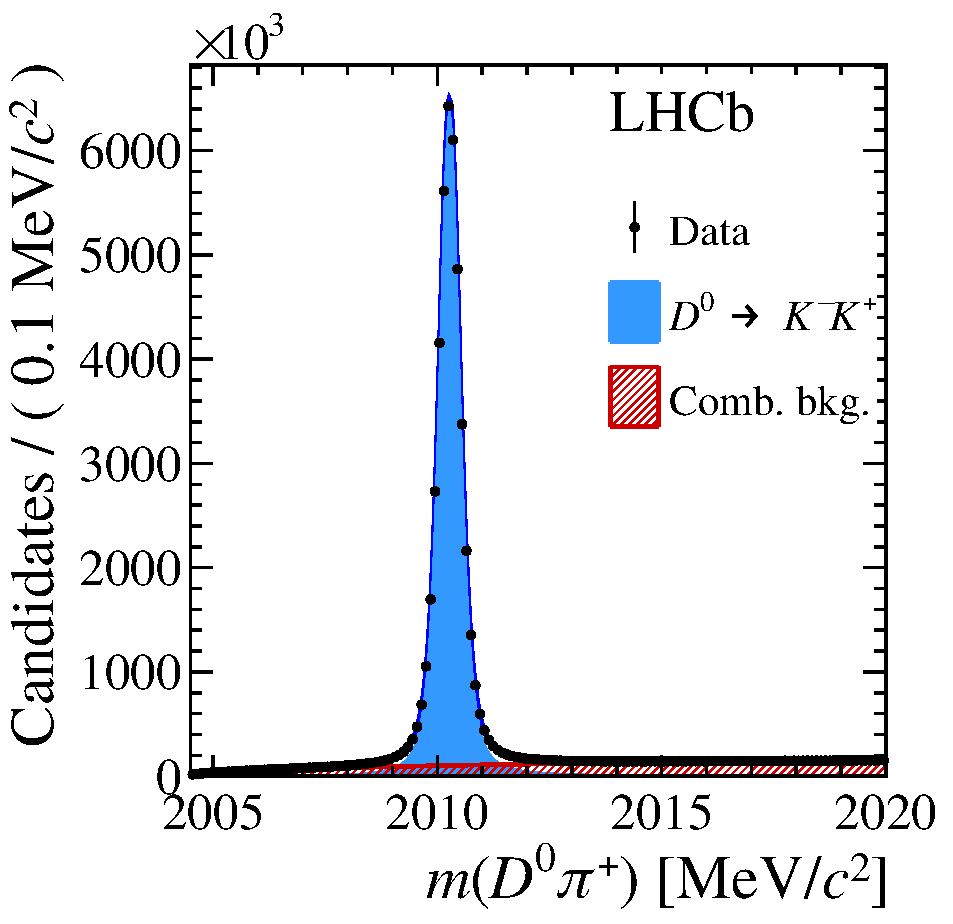
\includegraphics[width=.7\textwidth]{figures/charm_cpv_fit_pitagged_KK.pdf}
    \end{column}

    \begin{column}{.5\textwidth}
      \centering
            \textbf{\Ppiplus\Ppiminus final states}
      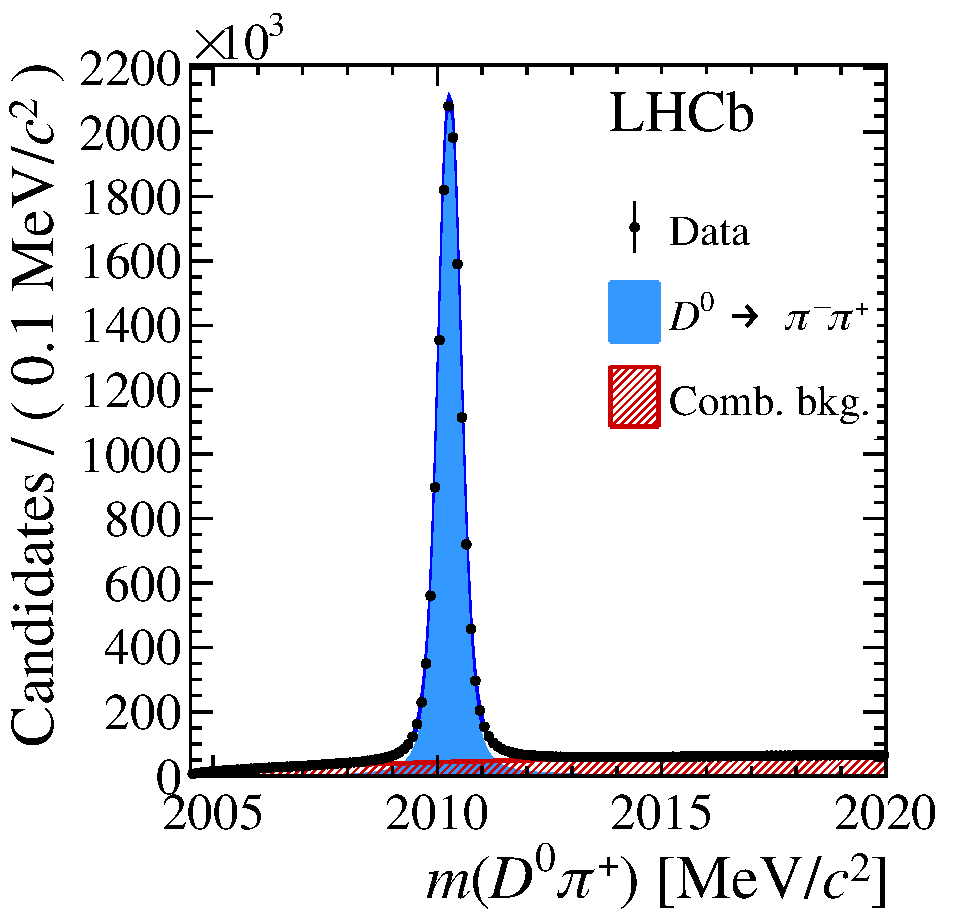
\includegraphics[width=.7\textwidth]{figures/charm_cpv_fit_pitagged_pipi.pdf}
    \end{column}
  \end{columns}
  \begin{itemize}
  \item 44 and 14 million \PKplus\PKminus and \Ppiplus\Ppiminus events, respectively
  \end{itemize}

\end{frame}

\begin{frame}
  \frametitle{Fit: \Pmu tagged}
  \begin{columns}
    \begin{column}{.5\textwidth}
      \centering
      \textbf{\PKplus\PKminus final states}
      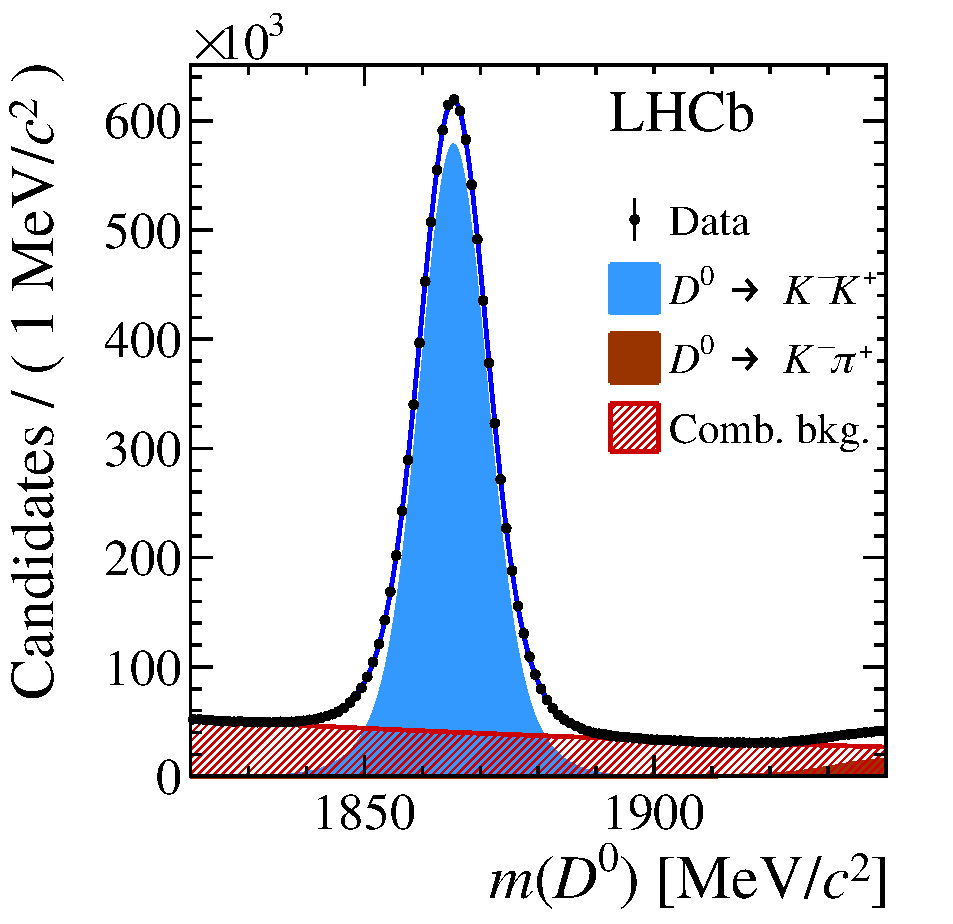
\includegraphics[width=.7\textwidth]{figures/charm_cpv_fit_mutagged_KK.pdf}
    \end{column}

    \begin{column}{.5\textwidth}
      \centering
            \textbf{\Ppiplus\Ppiminus final states}
      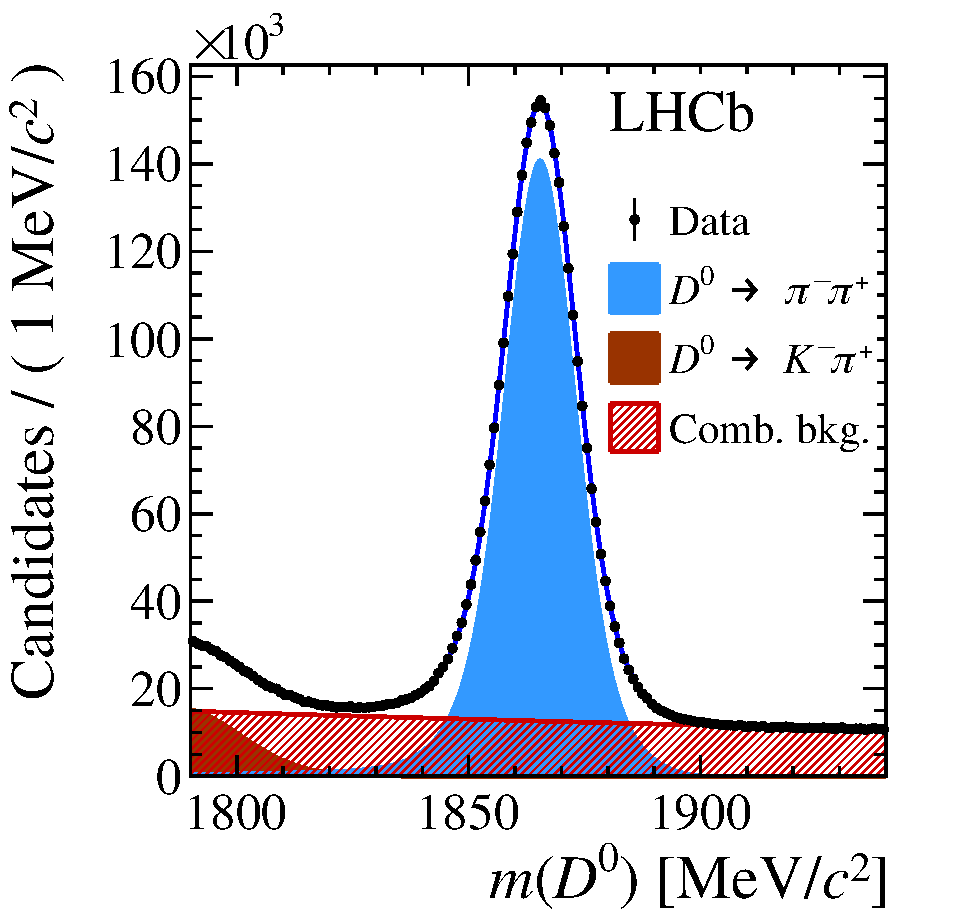
\includegraphics[width=.7\textwidth]{figures/charm_cpv_fit_mutagged_pipi.pdf}
    \end{column}
  \end{columns}
    \begin{itemize}
  \item 9 and 3 million \PKplus\PKminus and \Ppiplus\Ppiminus events, respectively
  \end{itemize}
\end{frame}

\begin{frame}
  \frametitle{Systematic uncertainties}
  \begin{columns}
    \begin{column}{.5\textwidth}
      \begin{itemize}
      \item \textbf{\Ppi-tagged systematics} dominated by
        \begin{itemize}
        \item fit model\\
          (from from fitting alternative models to toy-MC)
        \item misreconstructed background peaking in $m(\PDzero\Ppiplus)$ and not in $m(\PDzero)$\\
          (from yield and asymmetries of backgrounds on $m(\PDzero)$ distributions)
        \end{itemize}
      \item \textbf{\Pmu-tagged systematics} dominated by
        \begin{itemize}
        \item mistag: wrong muon\\
          from \PKminus\Ppiplus control sample
        \item \PB reconstruction efficiency as function of decay time between \PKplus\PKminus and
          \Ppiplus\Ppiminus, might worsen cancellation of $A_P$
        \end{itemize}
      \end{itemize}
    \end{column}

    \begin{column}{.5\textwidth}
      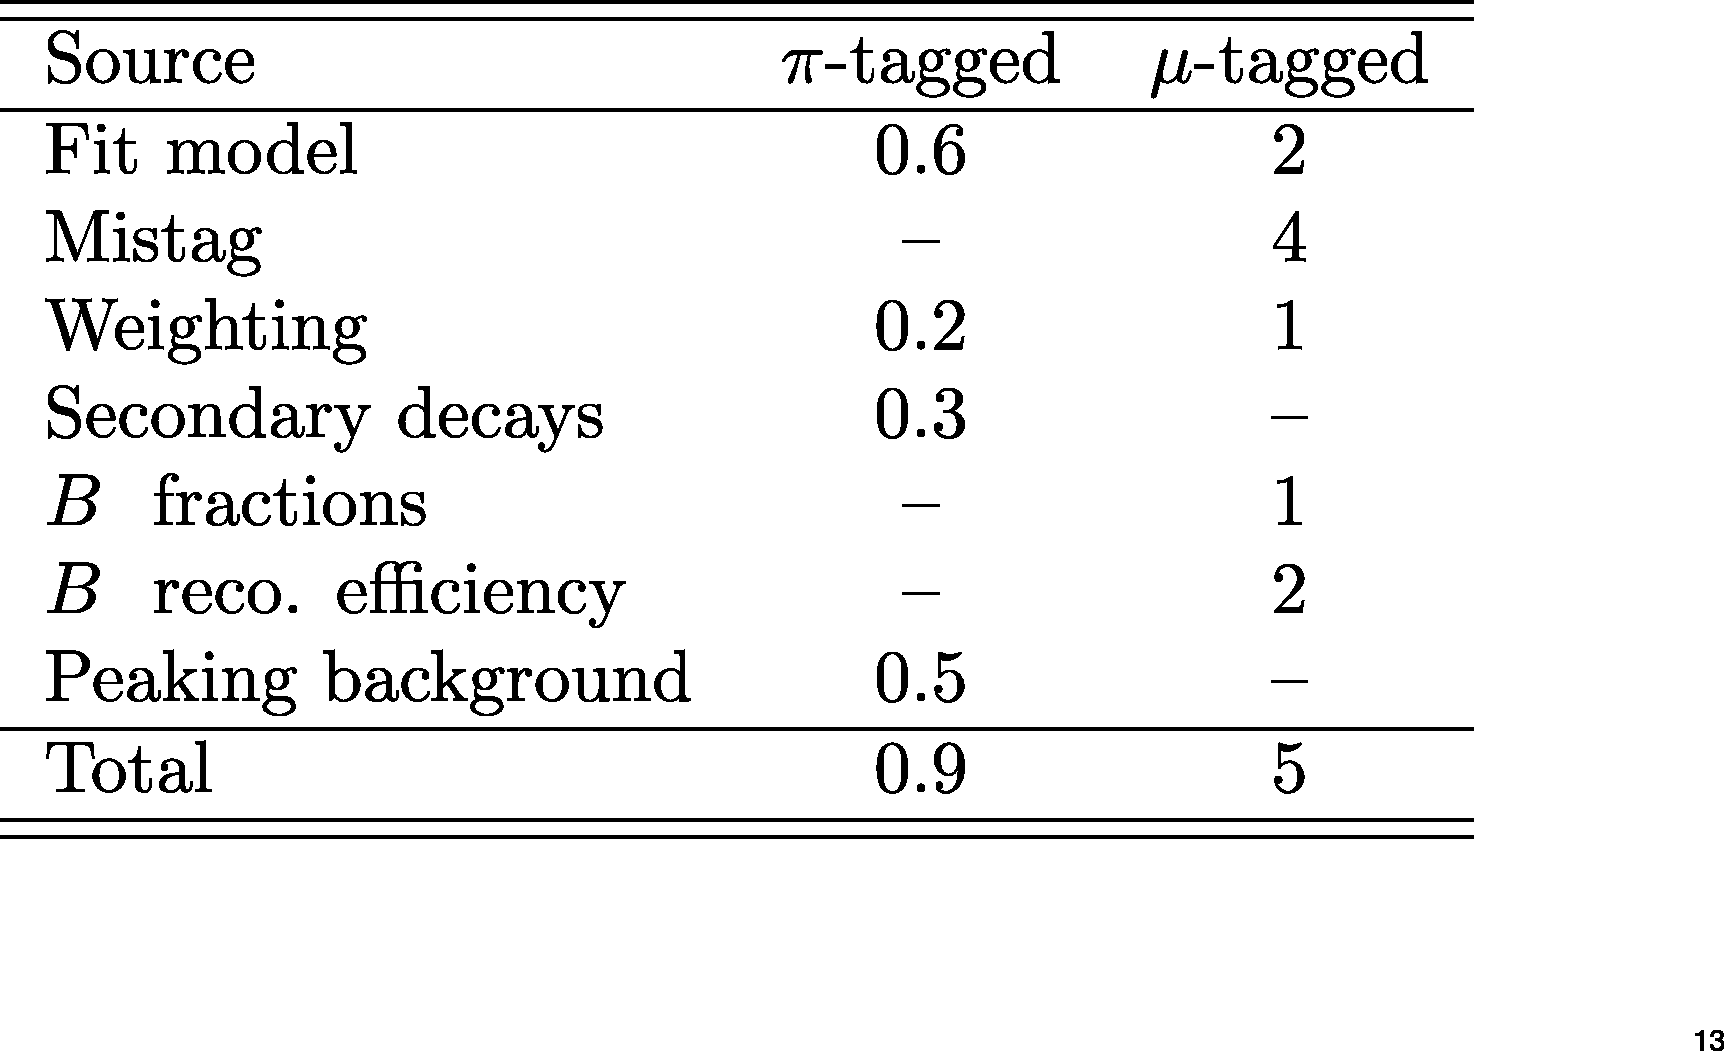
\includegraphics[width=\textwidth]{figures/charm_cpv_systematics.pdf}
    \end{column}
  \end{columns}
\end{frame}

\begin{frame}
  \frametitle{Results}
  \begin{eqnarray*}
    \Delta A_{CP}^{\Ppi-\mathrm{tagged}} & = & \left[-18.2 \pm 3.2 (\mathrm{stat.}) \pm 0.9
                                               (\mathrm{syst.} )\right] \times 10^{-4} \\
    \Delta A_{CP}^{\Pmu-\mathrm{tagged}} & = & \left[-9 \pm 8 (\mathrm{stat.}) \pm 5
                                               (\mathrm{syst.} )\right] \times 10^{-4} \\
  \end{eqnarray*}

  \begin{block}{Combined}
    \begin{equation*}
          \Delta A_{CP} = \left(-15.4 \pm 2.9)\right) \times 10^{-4}
        \end{equation*}
        \begin{itemize}
        \item \textcolor{kit-red100}{5.3$\sigma$} significance for deviation from 0
        \item first observation of $CP$ violation in charm
        \end{itemize}
\end{block}

\end{frame}

\begin{frame}
  \frametitle{Results II and outlook}
  With $A_\Gamma$ and $\Delta <t>$ from LHCb averages and world average \PDzero lifetime:
\begin{equation*}
  \Delta a_{CP}^{\rm dir} = \left(-15.7 \pm 2.9\right) \times 10^{-4} \Rightarrow \text{mostly direct CPV}
\end{equation*}
\begin{itemize}
\item results at upper limit but compatible with SM
\item further measurements and theoretical improvements necessary
\end{itemize}
\end{frame}

\begin{frame}
  \frametitle{Thanks for listening}
  
\end{frame}


\end{document}

%%% Local Variables:
%%% coding: utf-8
%%% mode: LaTeX
%%% TeX-engine: default
%%% TeX-master: t
%%% fill-column: 100
%%% ispell-dictionary: "english"
%%% eval: (flyspell-mode 1)
%%% eval: (add-to-list 'TeX-outline-extra '("\\\\frametitle\\b" 7))
%%% End: